\documentclass[TFM.tex]{subfiles}

\begin{document}

%\hyphenation{equi-va-len-cia}\hyphenation{pro-pie-dad}\hyphenation{res-pec-ti-va-men-te}\hyphenation{sub-es-pa-cio}
\chapter{Little disks operad}
TENER EN CUENTA KONTSEVICH[6] Y PREGUNTAR A MURO LO QUE TENGO APUNTADO ENCUADRADO EN TAMARKIN

ESCRIBIR ALGO AQUÍ, INCLUYENDO ALGO DE QUE ALL MAPS ARE REQUIRED TO BE CONTINUOUS

REVISAR LA NOTACIÓN POR SI DEBERÍA SER MÁS CONSISTENTE EN LOS ÍNDICES DE LOS OPERADS


\section{Operads}
First we give the general notion of (topological) operad and some properties of this object.
% EN PRINCIPIO LO DEFINO EN TOP Y YA PREGUNTO SI HACE FALTA QUE SEA EN UNA MONOIDAL SIMÉTRICA. SI HACE FALTA, HACER UNA SECCIÓN DE CATEGORÍAS SIMÉTRICAS MONOIDALES. SI NO, CITAR A DONALD YAU CON QUE SE PUEDE DEFINIR CON MÁS GENERALIDAD
%\url{https://ncatlab.org/nlab/show/operad}
%
%NO PARECE QUE ESTA DEFINICIÓN CAPTURE LA COMPOSICIÓN DEL LITTLE DISKS OPERAD, PERO EN VERDAD SÍ, LO QUE FALTA ES RELLENA CON LA IDENTIDAD HASTA COMPLETAR LA ARIDAD DEL PRIMERO
An operad is a collection of suitably interrelated spaces $\CC(j)$, the points of which are to
be thought of as $j$-adic operations $X^j \to X$ for some topological space $X$. Precisely, we have the following definitions.

\begin{defi}\label{operadtop}
An \emph{operad} (also \emph{symmetric operad}) $\CC$ consists of topological spaces $\CC(j)$ for $j\geq 0$, with $\CC(0)$ a single point $*$, together with the following data:
\begin{enumerate}[(1)]
\item Continuous functions $\gamma : \CC(k) × \CC(j_1) × \cdots × \CC(j_k) \to \CC(j)$, $j =\sum_s j_s$, such that the
following associativity formula is satisfied for all $c\in \CC(k)$, $d_s \in \CC(js)$, and $e_t \in \CC(i_t)$:

\[\gamma(
\gamma(c; d_1, \dots , d_k); e_1, \dots , e_j) = 
\gamma(c; f_1, \dots , f_k),
\]
where $f_s = \gamma(d_s; e_{j_1+\cdots+j_{s−1}+1}, \cdots , e_{j_1+\cdots+j_s} )$, and $f_s = *$ if $j_s = 0$. These functions are usually called \emph{structure maps}.

\item An identity element $1 \in \CC(1)$ such that 
$\gamma(1; d) = d$ for $d \in \CC(j)$ and 
$\gamma(c; 1^k) = c$ for
$c \in \CC(k)$, $1^k = (1, \dots , 1) \in \CC(1)^k$.

\item A right operation of the symmetric group $\Sigma_j$ on $\CC(j)$ such that the following equivariance
formulas are satisfied for all $c\in \CC(k)$, $d_s \in \CC(j_s)$, $\sigma\in\Sigma_k$, and $\tau_s\in\Sigma_{j_s}$:
\[
\gamma(c\sigma; d_1, \dots , d_k) = 
\gamma(c; d_{\sigma^{−1}(1)}, \dots , d_{\sigma^{−1}(k)})\sigma(j_1, \dots , j_k)
\]
and 
\[
\gamma(c; d_1\tau_1, \dots , d_k\tau_k) = \gamma(c; d_1, \dots , d_k)(\tau_1\oplus\cdots\oplus\tau_k),
\] 
where $\sigma(j_1, \dots , j_k)$ denotes the
permutation of $j$ letters which permutes the $k$ blocks of letters determined by the given
partition of $j$ (a first block of $j_1$, a second one of $j_2$ letters and so on), and $\tau_1\oplus\cdots\oplus\tau_k$ denotes the image of $(\tau_1, \dots , \tau_k)$ under the evident inclusion of $\tau_{j_1} × \cdots × \tau_{j_k}$ in $\Sigma_j$.
%{1,2,...,j} se divide en bloques y se permuta ese conjunto 
\end{enumerate}
\end{defi}

%\url{https://en.wikipedia.org/wiki/Operad_theory}


\begin{defi}
A \emph{morphism} $\psi:\CC \to \CC'$ of operads is a sequence of $\Sigma_j$-equivariant maps  $\psi_j : \CC(j)\to \CC'(j)$ such that
 $\psi_1(1) = 1$ and the following diagram commutes:
 \[
 \begin{tikzcd}
\CC(k)\times \CC(j_1)\times\cdots\times \CC(j_k) \arrow[r, "\gamma"] \arrow[d, "\psi_k\times\psi_{j_1}\times\cdots\psi_{j_k}"'] & \CC(j) \arrow[d, "\psi_j"] \\
\CC'(k)\times \CC'(j_1)\times\cdots\times \CC'(j_k) \arrow[r, "\gamma"]                                                         & \CC'(j)                   
\end{tikzcd}\]
$\Sigma_j$-equivariancy means that $\psi_j(c\sigma)=\psi_j(c)\sigma$ for all $c\in \CC(j)$, $\sigma\in\Sigma_j$ and $j\geq 0$. 
\end{defi}



\url{https://ncatlab.org/nlab/show/symmetric+monoidal+category#as_algebras_over_the_little_cubes_operad}
% HABLAR ALGO DE ESTAS CATEGORÍAS PARA QUE TENGA MÁS SENTIDO GENERALIZAR LAS DEFINICIONES Y DAR UNA IDEA DE CÓMO SE DEFINEN LAS OPERADS EN ESAS CATEGORÍAS

ALOMEJOR HACER DIBUJITOS DE LOS AXIOMAS \url{https://en.wikipedia.org/wiki/Operad#\%22Little_something\%22_operads}


\section{Little disks operad}\label{little}

From now on, by ``disk'' we will mean ``open disk''. 
 
 Let $E_2(n)$ be the configuration space of $n$ disks $B(x_i,r_i)$ of center $x_i\in D^2$ and radius $r_i\in (0,1)$ (called \emph{little disks}) inside the standard unit disk viewed $D^2$ as a subspaces of $(D^2\times (0,1))^n$ whose points are of the form $((x_1,r_1),\dots, (x_n,r_n))$. By convention, $E_2(0)=\{*\}$. Note that $r_i$ must be such that the disk of center $B(x_i,r_i)\subset D^2$ without intersecting any other disk $B(x_j,r_j)$. 
 
 There is an obvious homotopy equivalence $E_2(n)\simeq \mathcal{M}_2(n)$ from $E_2(n)$ to the configuration space of $n$ points of $D^2$. This homotopy equivalence is given by ``forgetting the radius'' of each little disk. Hence $\pi_1(E_2(n))\cong PB_n$, the pure braid group of order $n$, and $\pi_i(E_2(n))=0$ for $j>1$. 
 
 
\definecolor{xdxdff}{rgb}{0.49019607843137253,0.49019607843137253,1.}

\begin{figure}[h!]
\resizebox{10cm}{4.7cm}{%
\begin{tikzpicture}[line cap=round,line join=round,>=triangle 45,x=1.0cm,y=1.0cm]
\clip(-5.5,-3.4) rectangle (9.5,3.4);
\draw [line width=2.pt,color=xdxdff,fill=xdxdff,fill opacity=0.10000000149011612] (2.,1.) circle (0.7823042886243178cm);
\draw [line width=2.pt,color=xdxdff,fill=xdxdff,fill opacity=0.10000000149011612] (3.,-1.) circle (1.100727032465361cm);
\draw [line width=2.pt,color=xdxdff,fill=xdxdff,fill opacity=0.10000000149011612] (4.48,1.46) circle (0.7496665925596522cm);
\draw [line width=2.pt] (3.,0.) circle (3.1622776601683795cm);
\draw [line width=2.pt] (2.,1.) circle (0.7823042886243178cm);
\draw [line width=2.pt] (4.48,1.46) circle (0.7496665925596522cm);
\draw [line width=2.pt] (3.,-1.) circle (1.100727032465361cm);
\draw (1.84,1.3) node[anchor=north west] {$1$};
\draw (4.32,1.7) node[anchor=north west] {$2$};
\draw (2.8,-0.8) node[anchor=north west] {$3$};
\draw (-1.44,0.6) node[anchor=north west] {\LARGE{$c=$}};
\end{tikzpicture}
}
\caption{A point $c\in E_2(3)$.}
 \end{figure}
 

 
 
 We define for all positive integers $p$ and $q$ and  each $1\leq i\leq p$the composition or \emph{insertion} map 
 \[
 \begin{tikzcd}[row sep=10]
  E_2(p)\times E_2(q)\arrow[r, "\circ_i"] & E_2(p+q-1)\\
  (c_1,c_2)\arrow[r, mapsto, shorten <= 1em, shorten >= 1em] & c_1\circ_i c_2
 \end{tikzcd}
 \]
 by inserting $c_2$ inside $B(x_i,r_i)$ as shown in the figure. 
 
  
  \begin{figure}[h!]
  \centering
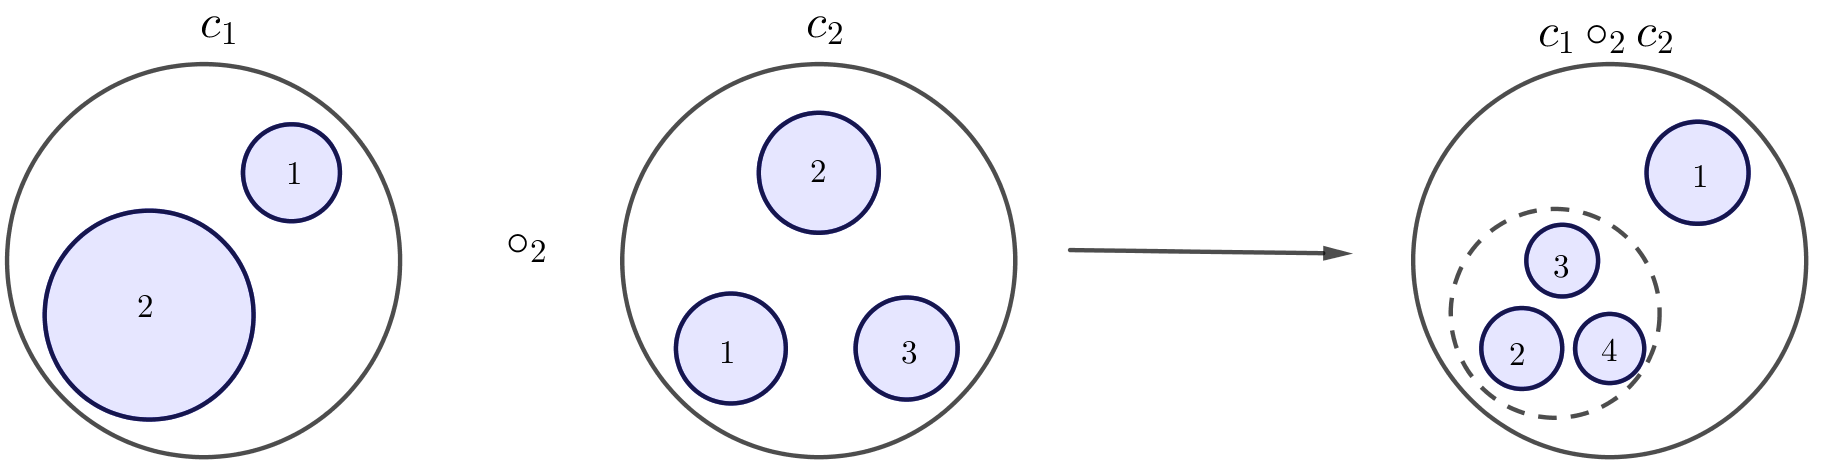
\includegraphics[scale=0.3]{Imagenes/insertion}
\caption{An insertion $\circ_2:E_2(2)\times E_2(3)\to E_2(4)$.}
 \end{figure}

Note that there is an element $Id_{E_2}\in E_2(1)$ given by the coordinates $(0,1)$ which acts as the identity for this map. It is easy to check that these maps satisfy the associativity property of an operad. IGUAL DEBERÍA PONERME A COMPROBARLO Y ESCRIBIRLO It is not difficult to check that the maps $\circ_i$ are compatible with this action in the sense of equivariance of operads QUIZÁ DEBERÍA COMPROBARLO Therefore, the familty $E_2=\{E_2(n)\}_{n\geq 0}$ is an operad with identity $Id_{E_2}$ and composition map $\circ_i$. This is what we call the \emph{little disks operad}.

\begin{remark}
In the definition of the structure maps we're omitting the disks on which only the identity is acting. If we want to write it with the same notation as we defined operads, the maps should be $\circ_i:O(p)\times O(q)\times O(1)\times\cdots \times O(1)\to O(p+q-1)$. COMENTAR QUE ES HABITUAL POR LA ASOCIATIVIDAD, QUE PERMITE HACERLO DE DOS EN DOS (COMPROBARLO)
\end{remark}

There is an action $E_2(n)\times \Sigma_n\to E_2(n)$ of the symmetric group on $E_2(n)$ given by rearranging the little disks. An example is shown below.
EJEMPLO DE LA ACCIÓN



\subsection{Action of $E_2$ on a loop space}
Given a based space $(X,x_0)$, consider the loop space $\Omega^2(X)$ of based maps $(S^2, (1,0,0))\to (X, x_0)$. One can interpret this maps as maps $\overline{D}^2\to X$ taking the boundary $S^1$ of $\overline{D}^2$ to $x_0$, since they induce a well defined map $\overline{D}^2/S^1\cong S^2\to X$ and we can choose the quotient map to identify the class of $S^1$ in $\overline{D}^2/S^1$ with the point $(1,0,0)\in S^2$. 

Now we can define for $n\geq 1$ an action $E_2(n)\times (\Omega^2(X))^n\to \Omega^2(X)$ given by $(c,\gamma_1,\dots, \gamma_n)\mapsto c(\gamma_1,\dots, \gamma_n)$, where 
$c(\gamma_1,\dots, \gamma_n):c\to X$ is defined as $\gamma_i$ on $B(x_i,r_i)$ and to be constantly the base point $x_0$ outside the little disks. This map has the following immediate properties:
\begin{enumerate}
\item $Id_{E_2}(\gamma)=\gamma$ for all $\gamma\in \Omega^2(X)$.
\item For $c_1\in E_2(p)$ and $c_2\in E_2(q)$, 
$$(c_1\circ_i c_2)(\gamma_1,\dots, \gamma_{p+q-1})=c_1(\gamma_1,\dots, \gamma_{i-1}, c_2(\gamma_i,\dots, \gamma_{i+q-1}),\dots, \gamma_{p+q-1}).$$ COMPROBARLA
\item For $c\in E_2(n)$ and $\sigma\in\Sigma_n$, $(c\cdot \sigma)(\gamma_1,\dots,\gamma_n)=c(\gamma_{\sigma^{-1}(1)},\dots, \gamma_{\sigma^{-1}(n)})$. 
\end{enumerate}
Note that for $n=0$, there is only the map $E_2(0)\to\Omega^2(X)$ inducing $*\mapsto x_0$. 

The action described above turns $\Omega^2(X)$ into an \emph{$E_2$-álgebra}. A formal definition of this concept is given below in terms of the \emph{endomorphism operad}.


\begin{defi}
Let $X$ be a topological space and define the \emph{endomorphism operad} $\xi_X$ as follows. Let $\xi_X(j)$ be the space of based maps $X^j\to X$, $X^0=*$, and $\xi_X(0)$ the inclusion $*\to X$. The data are defined by:
\begin{enumerate}
\item $\gamma(f;g_1,\dots, g_k)=f(g_1\times\cdots\times g_k)$ for $f\in \xi_X(k)$ and $g_s\in\xi_X(j_s)$ such that $\sum_s j_s=j$.
\item The identity element $\mathbbm{1}\in\xi_X(1)$ is the identity map on $X$.
\item $(f\sigma)(y)=f(\sigma y)$ for $f\in\xi_X(j)$, $\sigma\in\Sigma_j$ and $y\in X^j$, where $\Sigma_j$ acts on $X^j$ by $\sigma(x_1,\dots, x_j)=(x_{\sigma^{-1}(1)},\dots, x_{\sigma^{-1}(j)})$. 
\end{enumerate}

Given a morphism of operads $O\to \xi_X$, we say that the pair $(X,O)$ is an \emph{$O$-algebra} (sometimes called \emph{$O$-space} \cite{May}).
\end{defi}


Note that giving a morphism $O\to \xi_X$ is equivalent to give a sequence of maps $O(k)\times X^k\to X$, so this definition is consistent with saying that $\Omega^2(X)$ is an $E_2$-algebra. In any other symmetric monoidal category the definition works just as fine performing the obvious substitutions, and the equivalence mentioned before remains true by the well-known andjunction $\Hom(X\otimes Y,Z)\cong\Hom(X,\Hom(Y,Z))$ REFERENCIARLA EN ALGÚN LAO O PROBARLA. 

\url{https://ncatlab.org/nlab/show/algebra+over+an+operad}

NO SÉ DÓNDE PONER LA PARTE DE LAS CADENAS Y TODO ESO. EN CUANTO A ESO PREGUNTAR POR QUÉ SE COGÍA SOLO EL $E_2(2)$ (POR EL GRADO DE LA OPERACIÓN) Y CÓMO SE RELACIONA LA COHOMOLOGÍA DE HOCHSCHILD DE $A$ CON LA HOMOLOGÍA DEL LOOP SPACE (¿Y CUÁL ERA EL OBJETIVO DE ANALIZAR LA ACCIÓN ESA? ERA POR MOTIVACIÓN)

%PREGUNTARLE QUÉ SENTIDO TIENE SER QUASI-ISOMORFO A LA HOMOLOGÍA, SI LA HOMOLOGÍA DE LA HOMOLOGÍA ES 0
%
%CON LO DEL SUSTITUTO, SI TIENE LA MISMA HOMOLOGÍA QUE C2, ENTONCES CONSIGUES QUE C(SUSTITUTO) ACTÚE EN H(A,A), PERO DE AHÍ EN PRINCIPIO NO SE SACA LA ACCION EN C(A,A)
\subsection{Little $k$-disks operad}\label{intervals}

One can define an operad $E_k$ for $k\geq 0$ in the same way we've defined $E_2$, but replacing the 2-dimensional disks by $k$-dimensional disks. Their action on $\Omega^k(X)$ is defined similarly. For $k\geq 2$, $E_k$ gives rise to more topologically rich spaces, since they have non trivial homology groups in dimensions greater than $2$, and there is also an operad $E_\infty$ (see \cite{cuentas}). 

The case $k=1$ is particularly simple. For $E_1$, usually called \emph{little intervals operad}, we have the following proposition.

\begin{prop}\label{E1}
For all $n\geq 0$, $E_1(n)$ is a contractible space.
\end{prop}
\begin{proof}
The case $n=0$ is trivial so take $n>0$. We have that $E_1(n)\simeq \mathcal{M}_1(n)$ via the analogue of homotopy equivalence $E_2(n)\simeq\mathcal{M}_2(n)$.  Therefore, we've reduced the proof to show that the configuration space of $n$ points of $(0,1)$, $\mathcal{M}_1(n)$, is contractible. Any point $(x_1,\dots, x_n)\in\mathcal{M}_1(n)$ is a sequence of distinct points of $(0,1)$, so we can order them and consider the sequence $0<x_{i_1}<\cdots<x_{i_n}<1$. Let $p=\left(\frac{1}{n+1},\dots, \frac{n}{n+1}\right)\in \mathcal{M}_1(n)$. We show that $\mathcal{M}_1(n)\simeq \{p\}$. To do that is enough to show that the map $q:\mathcal{M}_1(n)\to \{p\}$ defined coordinatewise by $x_{i_k}\mapsto \frac{k}{n+1}$ is an homotopy equivalence. We define a homotopy $E_1(n)\times [0,1]\to E_1(n)$ coordinatewise as $x_{i_k}\mapsto (1-t)x_{i_k}+t\frac{k}{n+1}$ for each $t\in [0,1]$. Since $(0,1)$ is convex, this map is well-defined as a map of points of $(0,1)$. We need to check that it preserves the order. That's easy since if $x_{i_j}<x_{i_k}$, then clearly 
\[
(1-t)x_{i_j}+t\frac{j}{n+1}<(1-t)x_{i_k}+t\frac{k}{n+1}
\] 
Continuity if obvious and we've defined a homotopy from the identity map on $E_1(n)$ to $i\circ q$, where $i:\{p\}\hookrightarrow \mathcal{M}_1(n)$ is the inclusion. 
\end{proof}







%ESTO ES INTERESANTE, LO DEJO AQUÍ \url{https://amathew.wordpress.com/2011/11/13/operads-i/}

\section{Operads in symmetric monoidal categories}
We've treated operads only in the category of topological spaces, but they can be defined in a more general setting, namely, in any \emph{symmetric monoidal category} \cite{Yau}. We're going to introduce this categories since it becomes more natural to talk about operads and other constructions in other categories having that framework in advance.

\begin{defi}
A \emph{symmetric monoidal category} is a category $M$ equipped with:
\begin{enumerate}[(1)]
\item A functor $\otimes: M\times M\to M$ called the \emph{tensor product}.
\item An object $I\in M$ called the \emph{unit}.
\item Natural isomorphism $a_{x,y,z} : (x \otimes y) \otimes z \to x \otimes (y \otimes z)$ (called the \emph{associator}), $\lambda_x : I \otimes x \to x$ (\emph{left unitor}), $\rho_x : x \otimes I \to x$ (\emph{right unitor}) and $B_{x,y}: x\times y\to y\times x$ (\emph{braiding}).
\end{enumerate}

We then demand that the associator obey the pentagon identity, which says this diagram commutes:
\[
\begin{tikzcd}[column sep=-25, row sep=30]
                                                                                                            &                                                                     & (w\otimes x)\otimes (y\otimes z) \arrow[rrd, "{a_{w,x,y\otimes z}}"] &                                                                         &                                \\
((w\otimes x)\otimes y)\otimes z \arrow[rru, "{a_{w\otimes x,y,z}}"] \arrow[rdd, "{a_{w,x,y}\otimes 1_z}"'] &                                                                     &                                                                      &                                                                         & w\otimes(x\otimes(y\otimes z)) \\
                                                                                                            &                                                                     &                                                                      &                                                                         &                                \\
                                                                                                            & (w\otimes (x\otimes y))\otimes z \arrow[rr, "{a_{w,x\otimes y,z}}"] &                                                                      & w\otimes ((x\otimes y)\otimes z) \arrow[ruu, "{1_w\otimes a_{x,y,z}}"'] &                               
\end{tikzcd}
\]
We demand that the associator and unitors obey the triangle identity, which says this diagram commutes:
\[
\begin{tikzcd}
(x\otimes I)\otimes y \arrow[rr, "{a_{x,I,y}}"] \arrow[rd, "\rho_x\otimes 1_y"'] &            & x\otimes (I\otimes y) \arrow[ld, "1_x\otimes\lambda_y"] \\
                                                                                 & x\otimes y &                                                        
\end{tikzcd}
\]
We demand that the braiding and associator obey the hexagon identity:
\[
\begin{tikzcd}
(x\otimes y)\otimes z \arrow[r, "{a_{x,y,z}}"] \arrow[d, "{B_{x,y}\otimes 1_z}"'] & x\otimes (y\otimes z) \arrow[r, "{B_{x,y\otimes z}}"]   & (y\otimes z)\otimes x \arrow[d, "{a_{y,z,x}}"] \\
(y\otimes x)\otimes z \arrow[r, "{a_{y,x,z}}"]                                    & y\otimes (x\otimes z) \arrow[r, "{1_y\otimes B_{x,z}}"] & y\otimes (z\otimes x)                         
\end{tikzcd}
\]
And lastly, we demand that $B_{y,x}B_{x,y}=1_{x\otimes y}$.
\end{defi}

If we drop the braiding from the definition above we obtain what is simply called a \emph{monoidal category}.

\begin{ex}\
\begin{enumerate}
\item The categories $\Set$ and $\Top$ are symmetric monoidal categories with the cartesian product as tensor product and a singleton as unit. 
\item For $k$ some field, the category $\Vect_k$ of $k$-vector spaces carries the standard structure of a monoidal category coming from the tensor product, over $k$, of vector spaces. The standard braiding that identifies $V\otimes W$ with $W\otimes V$ by mapping homogeneous elements $v\otimes w$ to $w\otimes v$ obviously makes $\Vect_k$ into a symmetric monoidal category. 

\item The category $\Cat$ of small categories (the collection of objects and the collection of morphisms are both sets) is symmetric monoidal with the product of categories and the category of one object and only the identity morphism as unit.

\end{enumerate}
CHAIN COMPLEXES \url{https://ncatlab.org/nlab/show/tensor+product+of+chain+complexes} LA FORMAN SIN SYMMETRIC (PERO LO ES PORQUE OBJETO A OBJETO LO ES) PERO NO TENGO CLARO CUÁLES SON LAS DIFERENCIALES DEL COMPLEJO UNIDAD. A LAS OPERADS AQUÍ SE LE LLAMAN DG-OPERAD (DIFFERENTIAL GRADED) \url{https://ncatlab.org/nlab/show/dg-operad}


SIMPLICIAL SETS

SI ME HACE FALTA HABLO DE MÓDULOS Y DE ÁLGEBRAS


\end{ex}

(LAX) MONOIDAL FUNCTORS \url{https://ncatlab.org/nlab/show/monoidal+functor}

For an arbitrary symmetric monoidal category $\DD$ we obtain the following definition of operad, which specializes to the definition \ref{operadtop} for $\DD=\Top$.

\begin{defi}
COGER DE YAU, EN NLAB VIENE INCOMPLETO Y NO APARECEN MORFISMOS \url{https://ncatlab.org/nlab/show/operad}

LA DUDA SOBRE LA UNIDAD. COMO SE COGE UNA APLICACIÓN, CREO QUE BASTA DECIR QUE A LA UNIDAD LE ASOCIAS EL QUE HEMOS COGIDO COMO IDENTIDAD
\end{defi}
\end{document}

%isotopía \url{https://link.springer.com/chapter/10.1007%2F978-94-015-9319-9_6}
%Orientation preserving (que las cartas conservan la orientación) https://math.stackexchange.com/questions/1319234/meaning-of-the-expression-orientation-preserving-homeomorphism 
%O sea, conserva la orientación como superficie